\documentclass{article}

\usepackage[utf8]{inputenc}
\usepackage{amsfonts}
\usepackage{amstext}
\usepackage{amssymb}
\usepackage{bm}
\usepackage{xcolor}   
\usepackage[hidelinks]{hyperref}
\usepackage{amsmath}
\usepackage{enumerate}

\usepackage{booktabs,caption}
\usepackage{threeparttable}
\usepackage{adjustbox}
\usepackage{parskip}
\usepackage{color, colortbl}

\usepackage{todonotes}


% \usepackage[style=authoryear-comp,citestyle=numeric,maxcitenames=1,backend=biber]{biblatex}
\usepackage[style=numeric,citestyle=numeric,backend=biber,sorting=none]{biblatex}
\addbibresource[]{../sparse.bib}


\graphicspath{ {../ims/} }

\newcommand{\citetemp}[1]{(#1)}
\newcommand{\reftemp}[1]{(#1)}

%math
\newcommand{\vct}[1]{\bm{#1}} % vector symbol formatting 
\newcommand{\mtx}[1]{\bm{#1}} % matrix symbol formatting
\newcommand{\vnorm}[1]{||#1||}
\newcommand{\vunit}[1]{\hat{#1}}
\newcommand{\mskew}[1]{\tilde{#1}}
\newcommand{\pderiv}[2]{\frac{\partial#1}{\partial#2}}
\newcommand{\rpm}{\raisebox{.2ex}{$\scriptstyle\pm$}}
\newcommand{\mean}[1]{\langle{#1}\rangle} 

\newcommand{\citetodo}{[]}
\newcommand{\reflater}{{\color{red} \{ref\}}}

%my operators
\DeclareMathOperator{\fskew}{skew}
\DeclareMathOperator{\Project}{Project}

\title{Note: information theory of single cell trajectories}

\author{Daniel Barton}

\begin{document}

\maketitle


\newcommand{\dstep}{\ensuremath{\delta_{\text{step}}}}


\section{Problem Statement}

It is common to analyse systems of motile cells by single cell tracking experiments.
A tracking algorithm generally consists of image segmentation 
followed by a tracking algorithm that connects
points in a time series.

A general feature of emerging from such experiments is short timescale diffusive
behaviour and medium timescale persistent motion. (Unless gradients exist in
environment, we will assume that the long time behaviour will be undirected,
whether or not it is observed in the experimental time frame under consideration.)
A modified Furth equation has been presented to describe the mean squared displacement
of persistent random walks with short time diffusive behavior\cite{thomas2018instantaneous},

\begin{equation}
    \langle| \Delta\vct{r}|^2\rangle 
    = 4D\left( \frac{\Delta t}{1 - S} - P(1 - e^{-\Delta t/P}) \right) \, ,
\end{equation}
where $S$  is the fraction of the persistence time $P$ at which
the trajectory becomes superdiffusive, D is the diffusion coefficient.


Estimating the measurement error of the center of mass position in tracking 
data indicates that measurement error alone cannot explain the short time
diffusive behaviour\cite{thomas2018instantaneous}. This additional 
``biological noise'' is a consequence of the stochastic processes that 
drive cell motility and contains quantitative information about those processes.
For Eukaryotes these processes typically involve remodelling of the
actin cyctoskeleton, while for the twitching bacteria P. Aeruginosa, 
the formation, growth, attachement and retraction of type IV pili (TFP) are the 
stochastic processes driving motility.

For an isolated image, the position of the perimeter of the cell has 
an uncertainty of at least $\pm 0.5$ pixel size. In principle, 
aggregate measurements such as the center of mass can be determined with
sub-pixel precision. Jin~et~al. estimate the spatial resolution
of the two point tracking of spherocylindrical P. Aeruginosa bacterium to be
$0.03 \mu m$ (pixel size $0.06\mu m$)\cite{jin2011bacteria}. 
The time resolution of their imaging is $0.1s$ which indicates a lower bound
of approximately $0.3\mu m/s$ on the instantaneous velocities that can be accurately resolved. 
Under similar experimental procedures,
this bacteria typically has an average velocity of less than 
$0.1\mu m/s$\cite{ni2016bacteria}. In order to accurately resolve slower displacements
of the cell, Jin~et~al. coarse grain their trajectories according to a lengthscale 
of $\dstep = 0.12\mu m$ prior to further analysis.

This motivates the following question. How much information does the trajectory
contain about the subcellular processes involved before and after coarse graining?

% given that is difficult to distinguish between short time scale stochastic 
% processes and measurement noise, 

\section{Sample Entropy}

The sample entropy of a timeseries\cite{delgado2019approximate} is a measure
of its regularity, or equivalently, its randomness. For an embedding dimension $m$ it is 
the negative logarithm of the conditional probability that two sequences
which are similar for $m$ points are also similar for $m+1$ 
points\cite{richman2000physiological}. Similarity is normally determined by
the Chebyshev distance $d(\vct{x},\vct{y}) = \max(|x_i - y_i|) < r$ 
for some threshold $r$. The statstic can be written
$\text{SampEn}(m, r)$ and let its estimator for a sequence of length $N$
be $\text{SampEn}(m, r, N)$.

The sampling entropy is hindered by its dependence on both hyperparameters
$m$ and $r$, however its interpretation is greatly enchanced by 
its relative consistency that for two sequences $A, B$, and $r_1 \leq r_2$,
if 
$\text{SampEn}(m_1, r_1)(A) \leq \text{SampEn}(m_1, r_1)(B)$  
then
$\text{SampEn}(m_2, r_2)(A) \leq \text{SampEn}(m_2, r_2)(B)$.
The dependence of sample entropy on coarse graining 
has been referred to as multiscale sampling entropy (MSE)
and used to study heart rate data\cite{costa2002multiscale}
as well as other biological and non-biological processes. 

For a time series $\{x_1,\ldots,x_N\}$
we will use the coarse graining 
${ y_j = 1/\tau \sum_{i=(j-1)\tau+1}^{j\tau}, 1 \leq j \leq N/\tau }$,
which splits the trajectory into $j$ non-overlapping intervals 
of length $\tau$. 
The original trajectory is obtained for $\tau = 1$, 
we will not use the linearisation procedure that has previously been used to study
P. Aeruginosa tracking data because there is no equivalent well defined minimum displacment
(spurious results will be obtained if we allow the 
coarse graining length $\dstep \rightarrow 0$).

\begin{figure}[h]
    \centering
    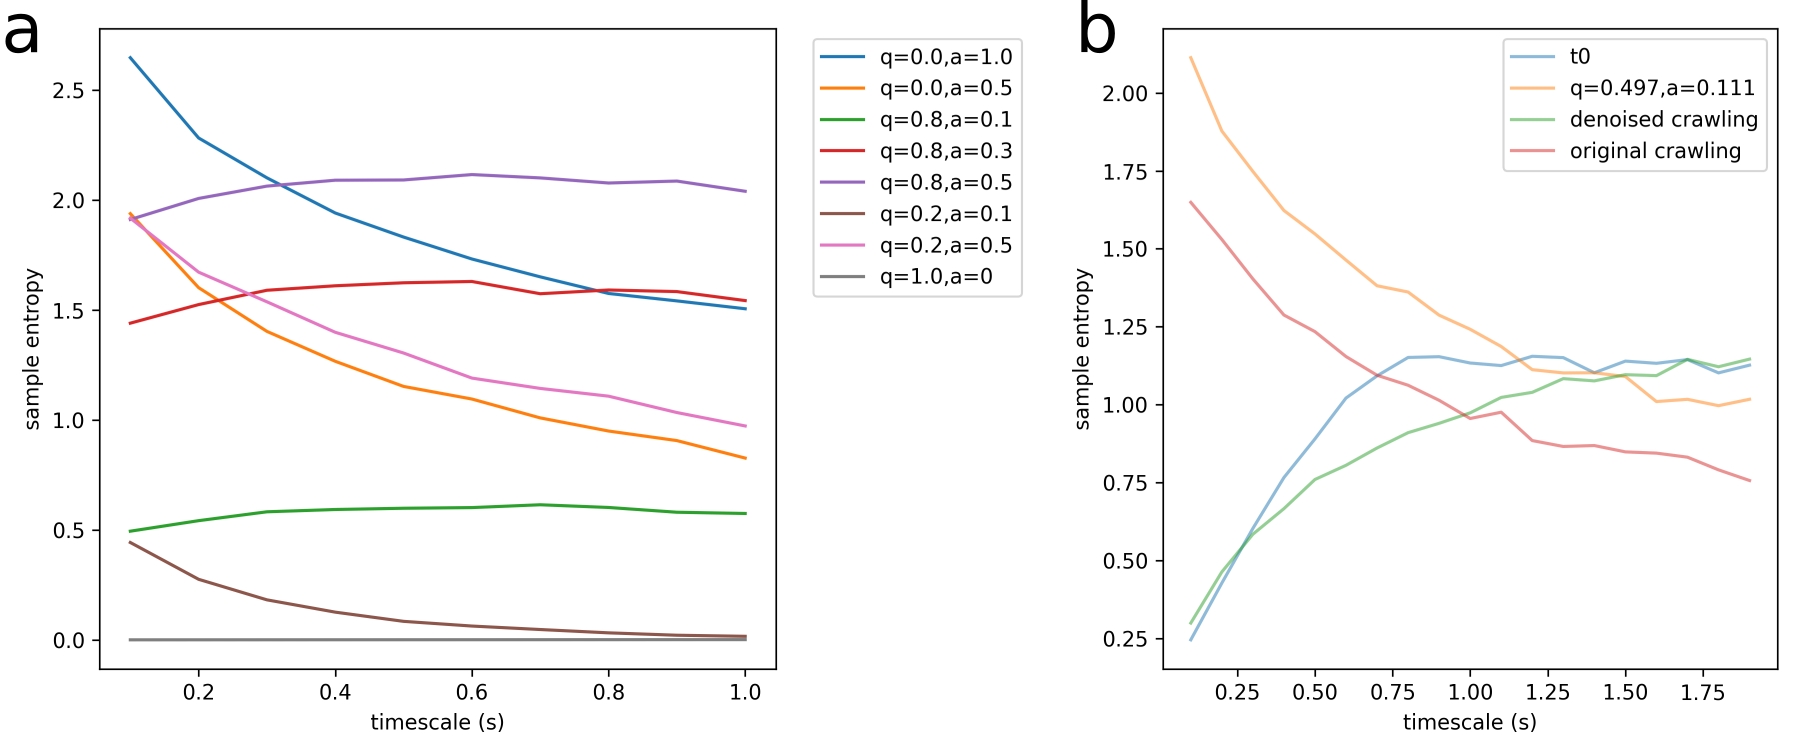
\includegraphics[width=0.9\textwidth]{composite_sample_entropy.png}
    \caption{
        (a) multiscale sample entropy of a 1d persistent random walk
        with various parameters.
        (b) multiscale sample entropy for persistent random 
        walk velocities and various twitching data. \textit{fanjin} refers to an ensemble
        of similar P.~Aeruginosa trajectories. t0 is simulated twitching data
        with parameters loosely determined by the real tracking data.
        linearised fanjin is the fanjin data linearised at $\dstep = 0.12\mu m$.
    }
    \label{fig:entropy}
\end{figure}

To quantify the information about biological processes that is retained after coarse graining
we will compare biological tracking data to a persistent random walk process
which is approximately similar to biological trajectories on 
long timescales\cite{dieterich2008anomalous,metzner2015superstatistical},
but is random at short timescales.
The persistent random walk is defined by two parameters $(q, a)$.
Velocity at the $i$th step is
$\vct{v}_i = q\vct{v}_{i-1} + a\vct{n}_i$, where
$a\vct{n}_i$ is a normally distributed random number with variance $a$.
We can use this model to generate arbitrarily long, biologically similar time series.
As such it might appear that the ``information content'' of such a trajectory is low.
That is not the kind of information that we are measuring with sample entropy. 
Sample entropy
is maximised for a purely random sample, in this case it 
is large when  $a/q$ is large. For $q = 0$ we recover ordinary white noise 
while for $a = 0$ we get an exactly predictable trajectory of minimum entropy.
The sampling entropy is shown against the coarse graining time $\tau$
for various choices of $q,a$ in figure~\ref{fig:entropy}.a, with $m=2$
and $r=0.2*SD$ where $SD$ is the standard deviation of the entire 
set of random data generated for all $(q,a)$ pairs. These are typical choices
of $m$ and $r$\cite{delgado2019approximate}. We restrict $N$ to be $10^4$
so that all sampling entropies can be computed in a few seconds.

We go on to compute SampEn for P. Aeruginosa tracking data and for a model of
twitching motility that is calibrated against this data. 
The tracking data is of 63 similar P. Aeruginosa crawling trajectories
with $0.1s$ time resolution. We again use $N = 10^4$ ($6.2\%$) of the 
available data.
We will compare against a persistent random 
walk with parameters $(q,a) = (0.50,0.11)$ obtained by using the 
simulated tracking data to calculate the maximum likelihood estimates for these parameters.
We previously used a one dimensional persistent random walk, here 
we generate 2d random walks and then compute the speed $u = |\vct{v}|$.

When comparing the sample entropy of time series, it is recommended to normalize 
these series by their standard deviations. We subsequently obtain $r$
as before by using 0.2$SD$ where $SD$ is the standard deviation over all
data being compared. The sample entropy of the persistent random walk model
increases on short timescales, just like white noise\cite{costa2002multiscale}.
Our twitching simulation does exactly the opposite, dropping sharply at low
$\tau$, reflecting the fact that on short timescales twitching is certainly not
random (Figure~\ref{fig:entropy}.b).
 TFP extension and retraction cycles are on the order of ~1s, 
at smaller timescales the dynamics depends on the exact configuration
of TFP as well as their binding and extension/retraction states.

% Despite being affected by an uncertain degree of experimental noise, the real tracking
% data follows a similar trend, this should motivate us to develop the tools
% to analyse the regularity of real biological trajectories at short timescales!

Sampling entropies for the persistent random walk model and smoothed or simulated twitching data converge 
at around 1.5s, giving us the expected limit at which the microscopic structure
of these biological trajectories is more or less washed out.
The unmodified crawling data obtained by segmentation and tracking follows the same
trend as the persistent random walk model, that is to say,
compared to the simulated twitching data it is highly random at short timescales. 
Given the spatial resolution of the microscope, we expect that
a significant portion of this randomness is due to measurement error
however real stochastic biological processes that are not captured by 
our choice of simplified model would also contribute.
The smoothed tracking data follows a similar trend to the simulated data,
however we have smoothed out biologically interesting features of the data and 
replaced it with a regular curve with short timescale properties that 
bear no relationship to the underlying mechanisms

Together, these results motivate us to expand our scope and examine the original tracking
data in more detail. By analysing the original tracking data, can we extract more meaningful
information about the underlying short timescale twitching dynamics.

\section{Minimum Description Length}

So far we have used tracking data which has been smoothed by a wavelet method
by Fan Jin lab. {\color{red} (Later we can smooth it again ourselves and gain control of the process.)}
We will start by using our ``candidate'' trajectory as example data, see figure~\ref{fig:candidate_track}. 
The trajectory was chosen because it has a very high mean velocity for this population but otherwise displays typical crawling motion.

\begin{figure}[h]
    \centering
    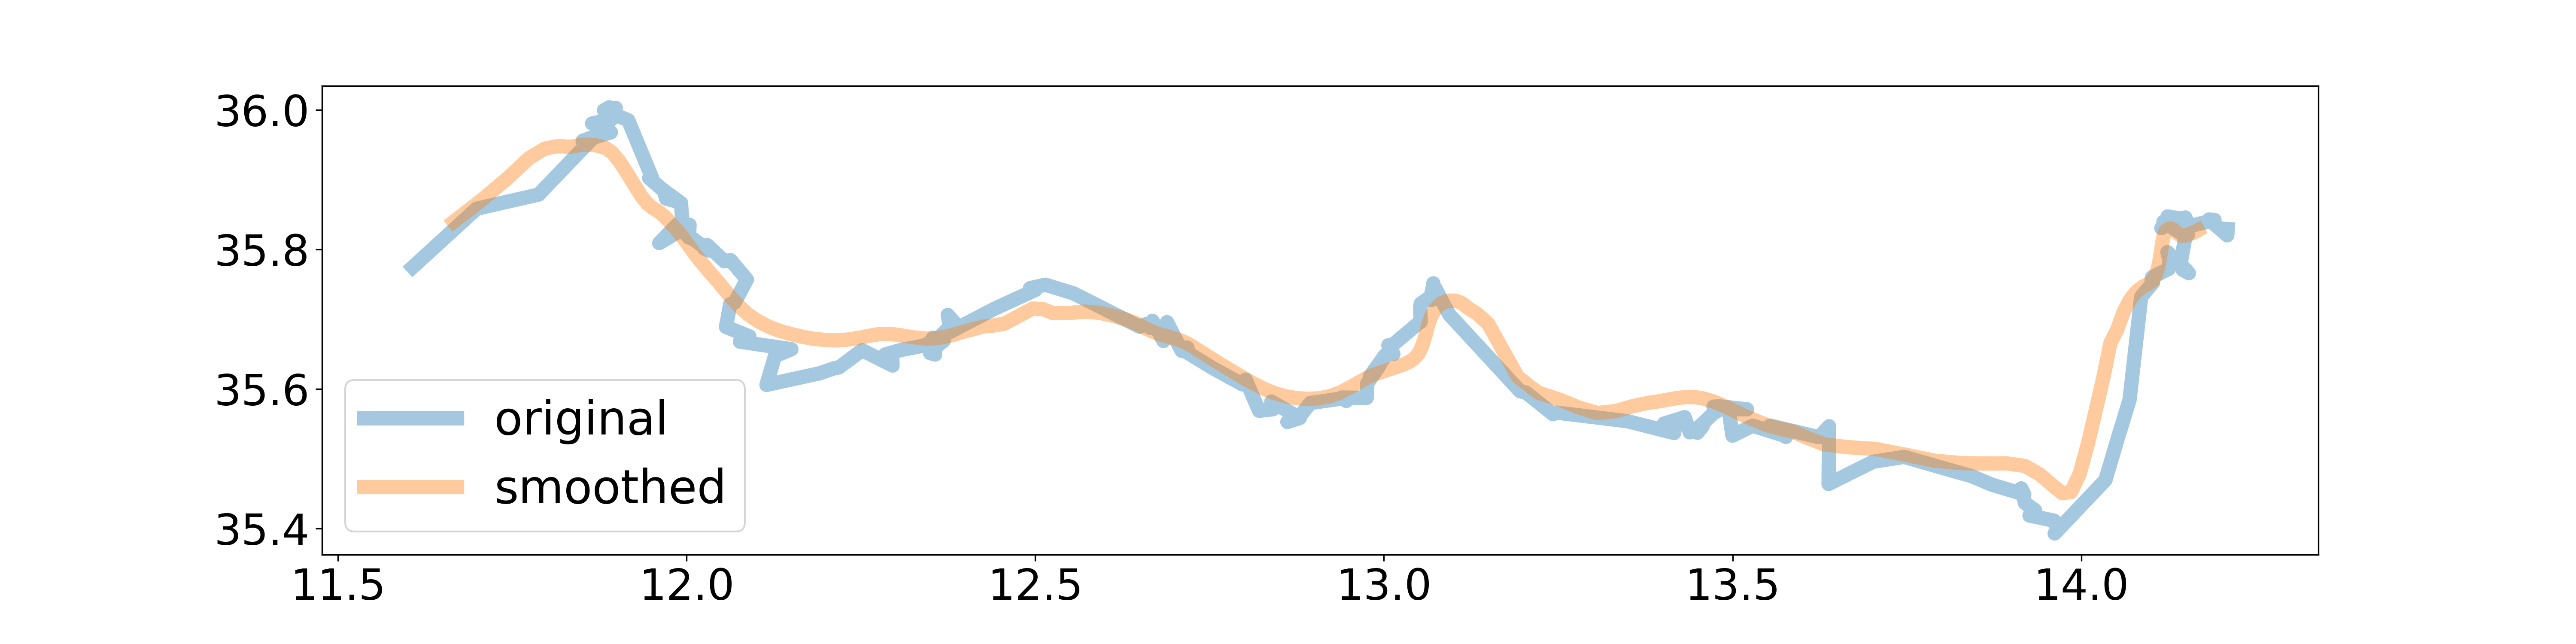
\includegraphics[width=0.9\textwidth]{example_track_data_20s.png}
    \caption{First 20 seconds (200 data points) of example trajectory, original tracking data (blue) and wavelet denoised (orange).
    }
    \label{fig:candidate_track}
\end{figure}

\newcommand{\vret}{v_{\mathrm{ret}}}
\newcommand{\tdwell}{\ensuremath{\tau_\text{dwell}}}

This track appears to contain some fast, linear displacements on the order of a few tenths of a micron.
In twitching data, it is natural to assoicate these displacements with the unconstrained retractions 
of one or more TFP. We assume that all translation of the bacteria is driven by TFP, hence we 
expect that the motion of the bacteria can be decomposed into short linear segments, corresponding
to TFP retraction events. 
Recent advances in direct observation of twitching motility with TFP visible 
show that TFP have a surface binding time of $\sim 1s$ and have typical extension and retraction
periods of several seconds\cite{tala2019pseudomonas,koch2021competitive}. 
Given $\vret$ is the typical TFP retraction velocity
and $\tdwell$ is the typical surface binding timescale, we expect the typical displacement distance
$\mean{d} \sim \vret \times \tdwell$, although for the purpose of this note
we consider this number to be unknown.
We do not see displacements with significant curvature, therefore we will neglect the possibility
that retraction of multiple TFP with varying speeds could lead to significantly curved paths.


Since the underlying TFP retraction mechanism generates approximately linear displacments, 
let us model our data as a piecewise linear trajectory described by a sequence of $M$ points $\left( \vct{x}_1^\prime,\ldots\,\vct{x}_M^\prime \right)$,
at corresponding time intervals $\left( t_1^\prime, \ldots, t_M^\prime \right)$. Let $N$ be the number of data points
in our tracking data.
This model is our data exactly for $M = N$, which we denote $\left( \vct{x}_1,\ldots\,\vct{x}_N \right)$,
for which the time intervals are constant $t_1 = \ldots = t_N = 0.1s$. 
If the cell makes linear displacements that are captured on multiple sequential timesteps,
we can replace this section of the trajectory with a single linear segment.
Equivalently we can search for piecewise linear models
with $M < N$ that still have a good fit to our original data.
Our goal is to obtain trajectories that are a better description of true underlying dynamics
than either the original noisy data or wavelet smoothed data.

For a fixed choice of $M$ we may attempt to solve an expensive global optimisation problem
using the least squares principle as our objective function.
Unfortunately a larger $M$ is always better for this optimisation,
and as $M\rightarrow N$ our piecewise linear model no longer provides any meaningful simplification of the data.
Rather than choose $M$ or penalize large values of $M$ in an ad hoc fashion, 
we will instead choose a ``coarsening'' length $l$ and use it to define a coarsening
procedure which operates on our tracking data to obtain a similar trajectory but with fewer segments. 
We sort the line segments by length and then
recursively remove the shortest segment $(\vct{x}_i,\vct{x}_{i+1})$ by 
replacing it with a single point $\vct{x}_i = (\vct{x}_i + \vct{x}_{i+1})/2$ until there are no segments 
with length less than $l$. The associated time intervals are also updated, e.g.  $t_i = t_i + t_{i+1}$.
Note that we can imagine many alternative coarsening procedures.
 For an appropriate choice of $l$, this procedure produces
piecewise linear models $\mathcal{M}(l)$ that appear to capture the main features of the original data but with
some degree of measurement noise smoothed out by the averaging procedure.
% We will come back to discuss this more rigorously after writing the least squares code

We turn again to the field of information theory in an effort to algorithmically discover 
an appropriate choice of $l$ (equivalently $M$). Specifically we are inspired by
the Minimum Description Length model selection princple 
as a way to choose $\mathcal{M}(l)$. This principle states that
the best model is the one which provides the shortest description of the data,
normally measured in bits.
Tracking data is composed of points where each point is a tuple of floating point numbers $(t,x,y)$,
we therefore define 1 unit of data as being a triple of floating point numbers (192 bits in our code).
Each measurement $(x,y)$ is random variable. In general random variables cannot be compressed,
however given a piecewise linear model $\mathcal{M}(l)$ we will consider points 
within a small separation $r$ of a line segment to be adequately described by the model
while the remaining $(\epsilon_1,\ldots,\epsilon_n)$ points are outliers and must be described separately.
The description length, $DL$, is
\begin{equation}
    DL(l) = DL(\mathcal{M}(l)) + DL(\epsilon_1,\ldots,\epsilon_n) = M(l) + n(l) \, . 
\end{equation}
The description length of the model is just $M$, the number of line segments it contains,
while the description length of the outliers is just $n$, their count. 
We have introduced a threshold parameter $r$, similar to the $r$ parameter used in the 
definition of sample entropy.

If the underlying trajectory is indeed composed, at least in part, of short linear displacements
with an unknown distribution and mean $\mean{d}$,
then we should expect to find that models obtained at some proportional coarsening length $l^\prime \sim \mean{d}$
are better (shorter) descriptions of the data than those for $l \ll l^\prime$, for which the model describes 
the measurement noise well but not the real trajectory and those for $l \gg l^\prime$ for which the model 
is too coarse grained to describe the real trajectory well. This result can be seen in figure~\ref{fig:description_length},
where for example using $r=0.01$, the minimum description length model has coarsening length $l = 0.031$.


\begin{figure}[h]
    \centering
    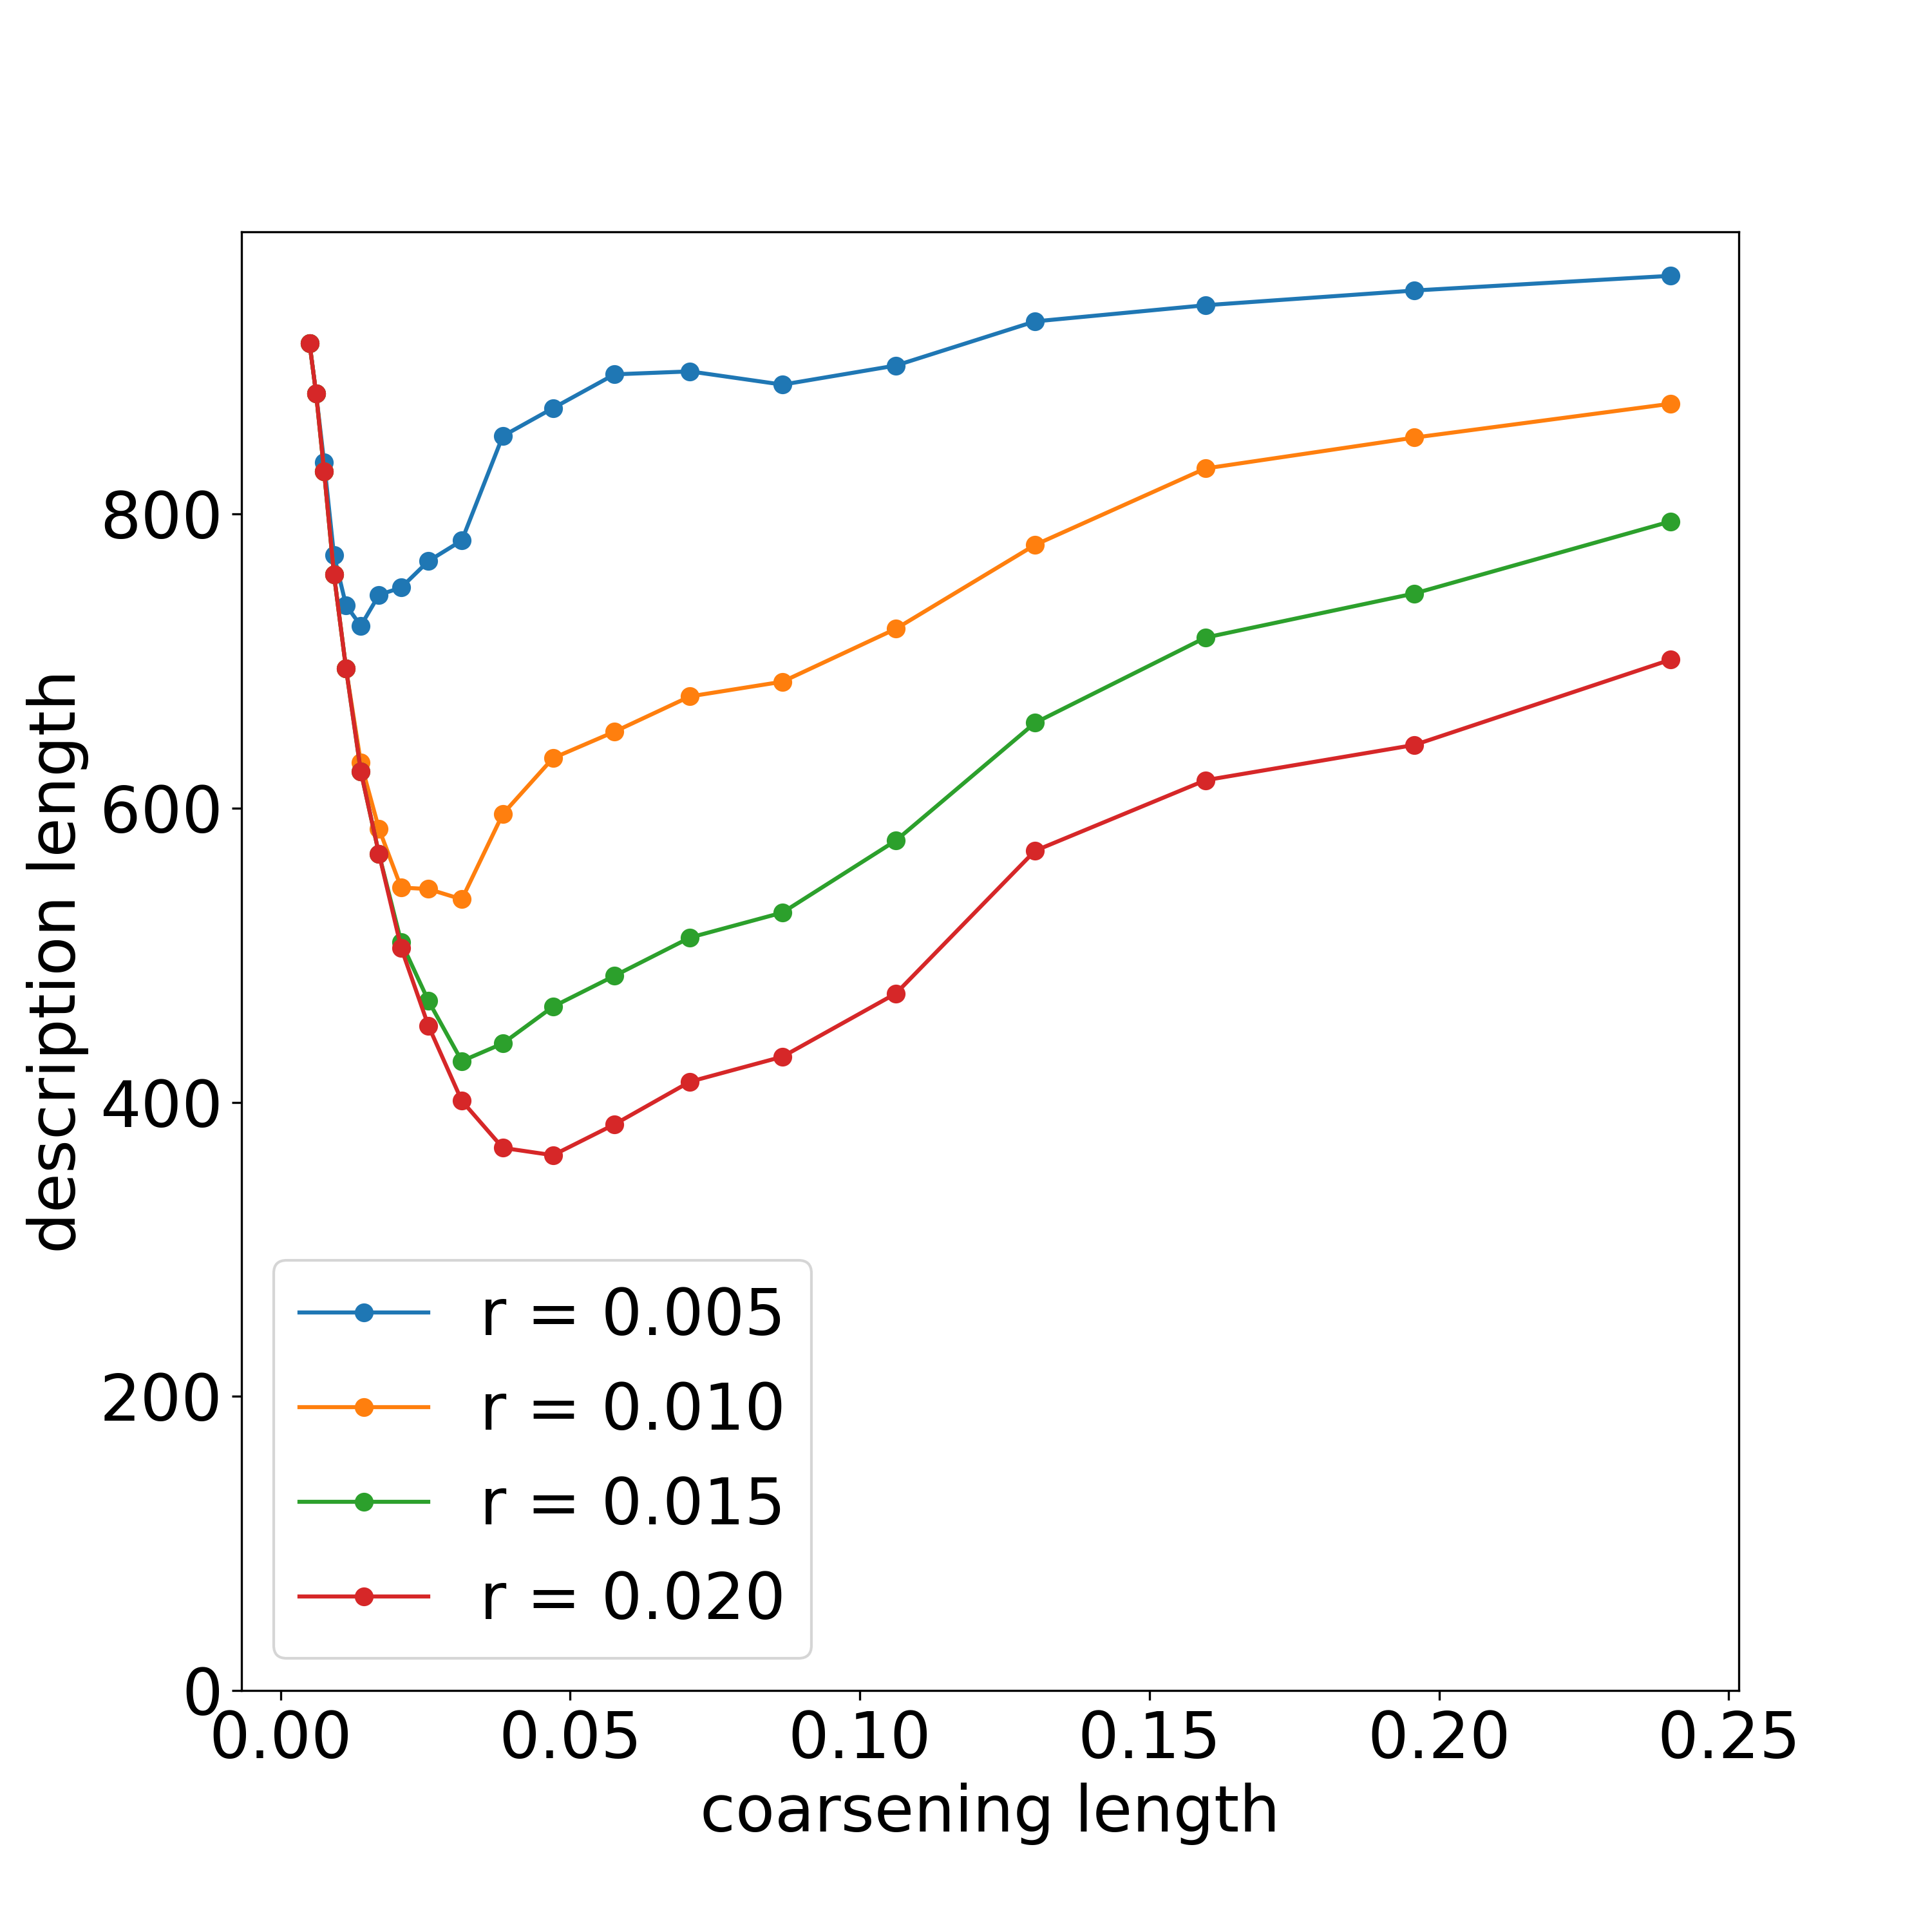
\includegraphics[width=0.5\textwidth]{description_length.png}
    \caption{Description length for varying coarsening length $l$ and threshold $r$
    }
    \label{fig:description_length}
\end{figure}

% TODO local optimisation




% The seperate problem of identifying the position of the vertices can be seen as a change point detection problem,
% algorithms have been developed to solve change point detection problems with varying numbers
% of changepoints up to a maximum number. 

\subsection{Optimisation}

We use the coarsening procedure to obtain initial guesses for the minimum description length model but 
we still need to search the vicinity of the initial guess for a locally optimal model.
Work in progress...

\begin{figure}[h]
    \centering
    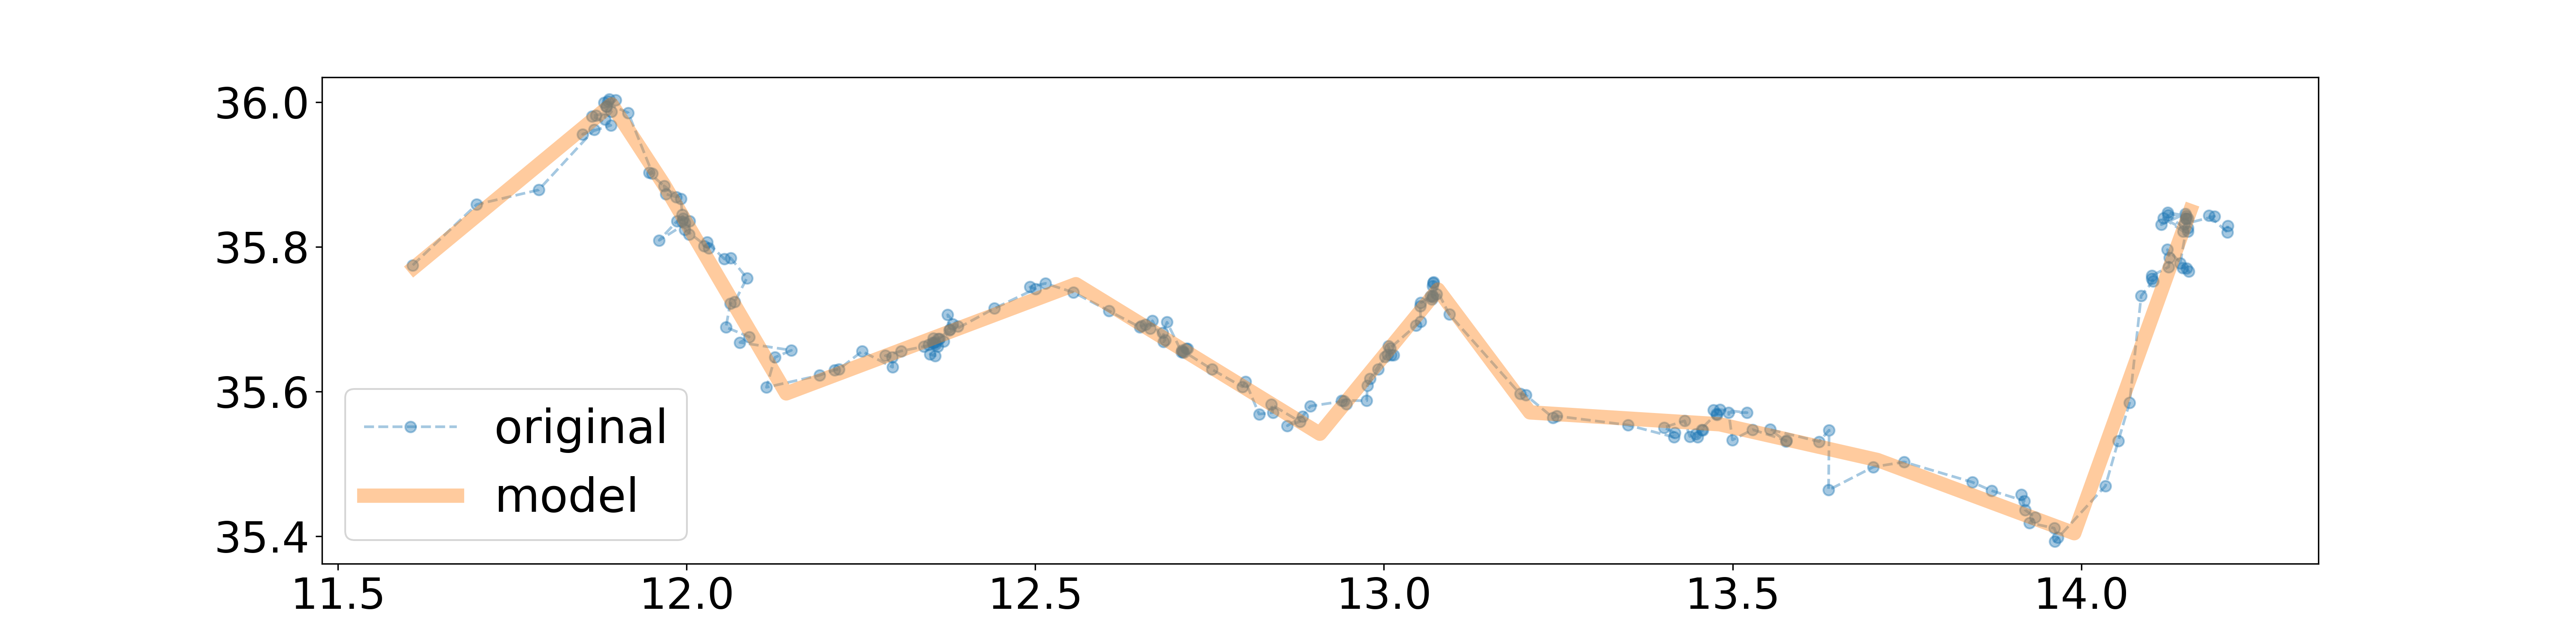
\includegraphics[width=0.8\textwidth]{candidate_short_mdlmodel.png}
    \caption{A Locally optimal model.  Pixel size $0.06\mu m$, $r = 0.03\mu m$, $l = 0.197\mu m$.
    }
    \label{fig:examplemodel}
\end{figure}


\subsection{Synthetic test data}

TODO

\subsection{Discussion}


%-----------------------------------------------------------------------

\medskip

\printbibliography

% =================================================================
\end{document}
% ------------------------------------------------------------------------
